\documentclass[11pt,aspectratio=169]{beamer}
\usepackage{imaxbeamer}

\title[F24 -- Kilder og randbetingelser]{Forelesning 24\\ Endelig volum i 1D: kildeledd og randbetingelser med kjent fluks}
\subtitle{Kompendium §3.5}
\author{IMAx3012 / IMAA3012 -- Matematikk 3B}
\date{}

\tikzset{
  node1d/.style={circle, fill=black, inner sep=0pt, minimum size=1.8mm},
  randpkt/.style={rectangle, draw=red!70!black, fill=red!30, inner sep=0pt, minimum size=2.4mm},
}

\begin{document}

\begin{frame}
\titlepage
\end{frame}

\begin{frame}{I dag}
\begin{remb}{Fra F23}
\[
a_P\phi_P = a_W\phi_W + a_E\phi_E + S^u, \qquad a_P = a_W + a_E - S_P
\]
Randverdier: kutt koblingen og legg bidraget i $S^u$ og $S_P$.
\end{remb}
\begin{enumerate}
\item Kildeleddet: lineær form $S^u + S_P\phi_P$ -- og hvorfor $S_P\le 0$.
\item Eksempel: plate med varmeproduksjon. Hvor kommer feilen fra?
\item Eksempel: ribbe som kjøles av luft (øving 7).
\item Randbetingelser med kjent fluks -- og isolert rand.
\end{enumerate}
\medskip
Kode til eksemplene finnes i \texttt{F24\_EVM\_1D\_Kilder\_Randbetingelser.ipynb} -- se gjerne på den.
\end{frame}

\section{Kildeleddet}

\begin{frame}{Kildeleddet integrert over kontrollvolumet}
\[
\frac{d}{dx}\left(\Gamma\frac{d\phi}{dx}\right) + S = 0
\quad\Longrightarrow\quad
\left(\Gamma A\frac{d\phi}{dx}\right)_e - \left(\Gamma A\frac{d\phi}{dx}\right)_w + \underbrace{\iiint_{KV} S\,dV}_{\approx\ \overline S\,A\,\delta x} = 0
\]
Kilden kan avhenge av $\phi$. Vi skriver den alltid på \emph{lineær} form:
\begin{oppsumb}{Linearisert kildeledd}
\[
\overline S\,\Delta V = S^u + S_P\,\phi_P
\]
\end{oppsumb}
\begin{itemize}
\item \textbf{Konstant kilde} $q$ (W/m$^3$): \quad $S^u = q\,A\,\delta x$, \quad $S_P = 0$.
\item \textbf{Sluk} $-n^2(T - T_\infty)$, konvektiv kjøling ($T_\infty$: omgivelsestemperatur, $n^2=\frac{hO}{\kappa A}$): \quad $S^u = n^2 T_\infty A\,\delta x$, \quad $S_P = -n^2 A\,\delta x$.
\item \textbf{Kjent randtemperatur} (F23): \quad $S^u = \frac{2\Gamma A}{\delta x}\phi_B$, \quad $S_P = -\frac{2\Gamma A}{\delta x}$.
\end{itemize}
\end{frame}

\begin{frame}{Hvorfor bør $S_P \le 0$?}
\begin{columns}[c]
\begin{column}{0.50\textwidth}
\begin{itemize}
\item $a_P = a_W + a_E - S_P \;\ge\; a_W + a_E$:\\ systemet blir \emph{diagonaldominant}.
\item Fysisk: et varmetap som \emph{øker} med $T$, demper temperaturen -- det stabiliserer.
\item Legg den $T$-avhengige delen av slukleddet i $S_P$, ikke i $S^u$.
\item Positiv $S_P$ kan gjøre $a_P$ liten eller negativ $\Rightarrow$ ustabilt og ufysisk.
\end{itemize}
\begin{remb}{Jacobi (høyre)}
\small Samme sluk, $n^2=25$: med $S_P<0$ konvergerer Jacobi; med alt i $S^u$ divergerer den -- i et sagtannmønster, som i F21.
\end{remb}
\end{column}
\begin{column}{0.48\textwidth}
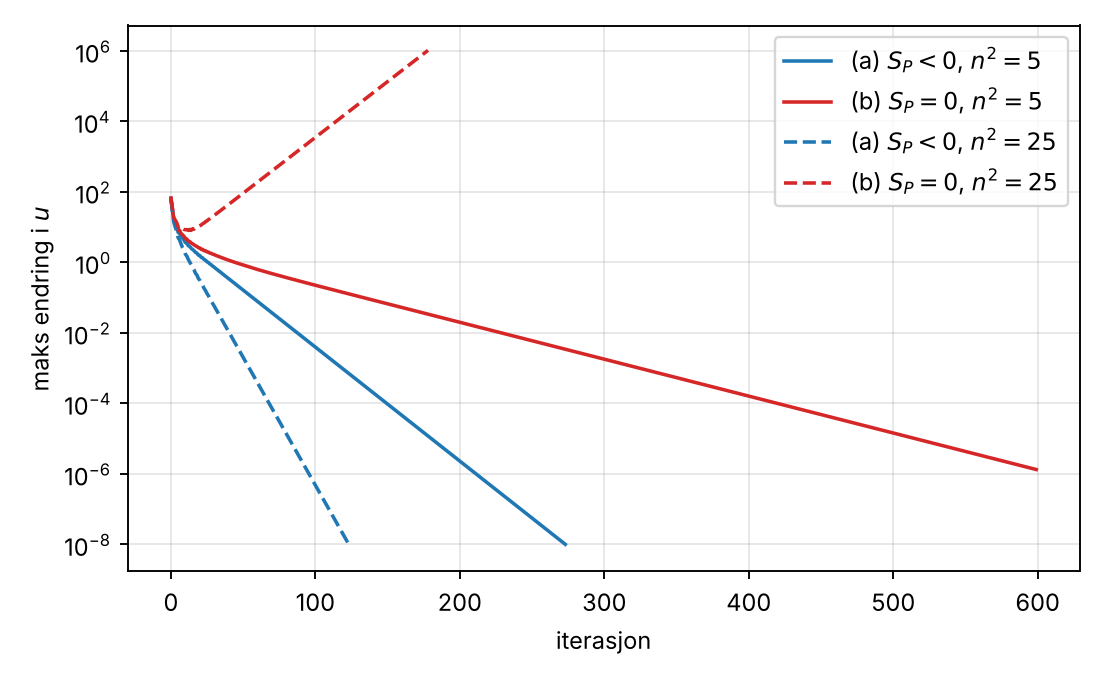
\includegraphics[width=\textwidth]{assets/sp_jacobi.png}
\end{column}
\end{columns}
\end{frame}

\section{Eksempel: plate med varmeproduksjon}

\begin{frame}{Eksempel: plate med jevn varmeproduksjon}
\begin{columns}[c]
\begin{column}{0.42\textwidth}
\centering
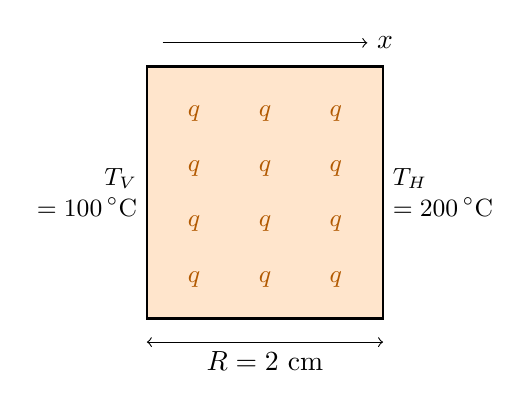
\begin{tikzpicture}[x=1cm,y=1cm]
\fill[orange!20] (0,0) rectangle (3,3.2);
\draw[thick] (0,0) rectangle (3,3.2);
\foreach \y in {0.5,1.2,1.9,2.6} \foreach \x in {0.6,1.5,2.4} \node[orange!70!black, font=\small] at (\x,\y) {$q$};
\node[left, align=right, font=\small] at (0,1.6) {$T_V$\\$=100\,^\circ$C};
\node[right, align=left, font=\small] at (3,1.6) {$T_H$\\$=200\,^\circ$C};
\draw[<->] (0,-0.3) -- (3,-0.3) node[midway, below] {$R = 2$ cm};
\draw[->] (0.2,3.5) -- (2.8,3.5) node[right] {$x$};
\end{tikzpicture}
\end{column}
\begin{column}{0.56\textwidth}
\[
\frac{d}{dx}\left(k\frac{dT}{dx}\right) + q = 0
\]
\begin{itemize}
\item $k = 0.5$ W/(m K), $q = 1000$ kW/m$^3$, $A = 1$ m$^2$.
\item Fem kontrollvolum: $\delta x = 0.004$ m.
\item $\dfrac{kA}{\delta x} = 125$, \quad $qA\,\delta x = 4000$.
\end{itemize}
Analytisk løsning:
\[
T(x) = \left(\frac{T_H - T_V}{R} + \frac{q}{2k}(R-x)\right)x + T_V
\]
\end{column}
\end{columns}
\end{frame}

\begin{frame}{Diskretiseringen -- les av $a_W$, $a_E$, $S^u$ og $S_P$}
\small
Integrer over hvert kontrollvolum og tilnærm fluksene lineært ($\delta x$ mellom noder, $\delta x/2$ til randen):

\medskip
\textbf{Indre node} $P = 2,3,4$:
\[
kA\frac{T_E - T_P}{\delta x} - kA\frac{T_P - T_W}{\delta x} + qA\,\delta x = 0
\;\;\Longrightarrow\;\;
\Big(\underbrace{\tfrac{kA}{\delta x}}_{a_W} + \underbrace{\tfrac{kA}{\delta x}}_{a_E}\Big)T_P
= \tfrac{kA}{\delta x}T_W + \tfrac{kA}{\delta x}T_E + \underbrace{qA\,\delta x}_{S^u}
\]
\textbf{Venstre randnode} $P = 1$ (kjent $T_V$, avstand $\delta x/2$):
\[
kA\frac{T_E - T_P}{\delta x} - kA\frac{T_P - T_V}{\delta x/2} + qA\,\delta x = 0
\;\;\Longrightarrow\;\;
\Big(\tfrac{kA}{\delta x} + {\color{red}\tfrac{2kA}{\delta x}}\Big)T_P
= 0\cdot T_W + \tfrac{kA}{\delta x}T_E + qA\,\delta x + {\color{red}\tfrac{2kA}{\delta x}T_V}
\]
\vspace{-2mm}
\begin{columns}[t]
\begin{column}{0.5\textwidth}
\begin{itemize}
\item Indre: $a_W = a_E = \frac{kA}{\delta x}$, $S^u = qA\,\delta x$, $S_P = 0$.
\item Rand: $a_W = 0$, $a_E = \frac{kA}{\delta x}$, $S^u = qA\,\delta x + {\color{red}\frac{2kA}{\delta x}T_V}$, $S_P = {\color{red}-\frac{2kA}{\delta x}}$.
\end{itemize}
\end{column}
\begin{column}{0.48\textwidth}
\begin{remb}{Alltid}
$a_P = a_W + a_E - S_P$. \; Node 5 er speilbildet av node 1 med $T_H$.
\end{remb}
\end{column}
\end{columns}
\end{frame}

\begin{frame}{Koeffisientene -- og matrisen $L$ og høyresiden $F$}
\begin{columns}[c]
\begin{column}{0.47\textwidth}
\centering\scriptsize
\setlength{\tabcolsep}{3pt}
\begin{tabular}{cccccc}
\toprule
Node & $a_W$ & $a_E$ & $S^u$ & $S_P$ & $a_P$ \\
\midrule
1 & 0 & 125 & $4000+250T_V$ & $-250$ & 375 \\
2 & 125 & 125 & 4000 & 0 & 250 \\
3 & 125 & 125 & 4000 & 0 & 250 \\
4 & 125 & 125 & 4000 & 0 & 250 \\
5 & 125 & 0 & $4000+250T_H$ & $-250$ & 375 \\
\bottomrule
\end{tabular}
\end{column}
\begin{column}{0.51\textwidth}
\scriptsize
\setlength{\arraycolsep}{2.5pt}
\[
\underbrace{\begin{bmatrix}
375 & -125 & & & \\
-125 & 250 & -125 & & \\
 & -125 & 250 & -125 & \\
 & & -125 & 250 & -125 \\
 & & & -125 & 375
\end{bmatrix}}_{L}
\begin{bmatrix} T_1\\T_2\\T_3\\T_4\\T_5 \end{bmatrix}
=
\underbrace{\begin{bmatrix} 29000\\4000\\4000\\4000\\54000 \end{bmatrix}}_{F}
\]
\end{column}
\end{columns}
\vspace{0.4em}
\begin{itemize}
\item Kilden gir $S^u = 4000$ i \emph{alle} nodene. Randnodene får i tillegg randbidraget fra F23.
\item I koden: \texttt{L} som i F23, og \texttt{F = q*A*deltax*np.ones(m)} pluss randleddene \texttt{kA/dx[0]*a} og \texttt{kA/dx[-1]*b}.
\end{itemize}
\end{frame}

\begin{frame}{Løsningen}
\begin{columns}[c]
\begin{column}{0.55\textwidth}
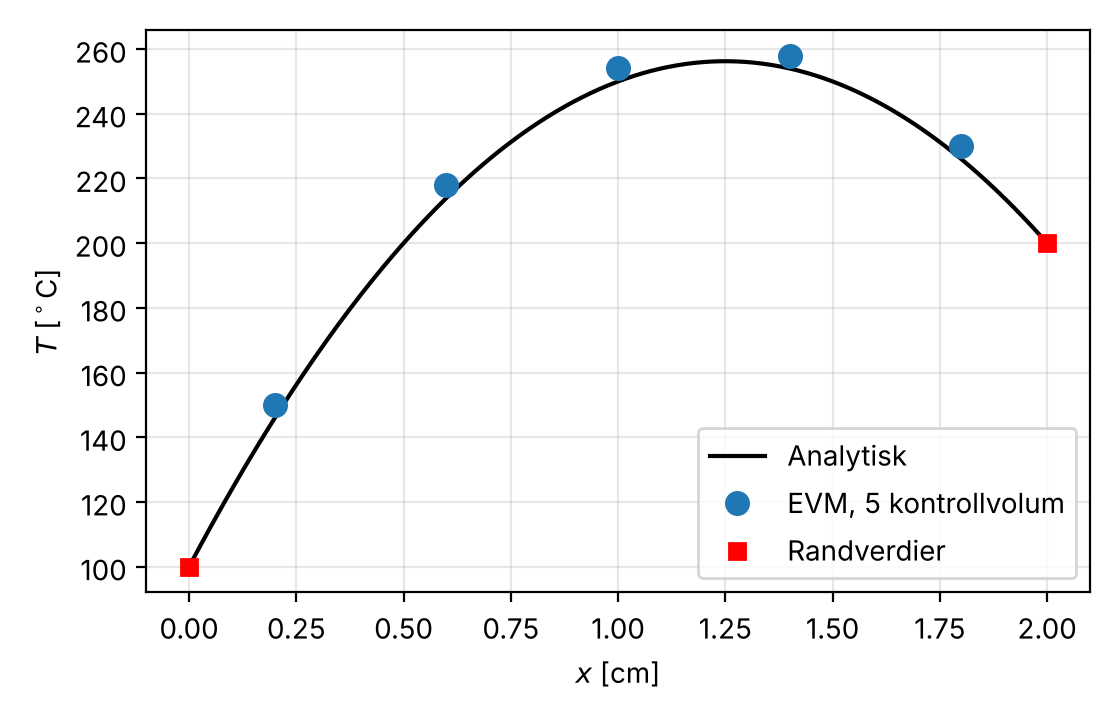
\includegraphics[width=\textwidth]{assets/plate_losning.png}
\end{column}
\begin{column}{0.43\textwidth}
\centering\small
\begin{tabular}{ccc}
\toprule
Node & EVM & Analytisk \\
\midrule
1 & 150 & 146 \\
2 & 218 & 214 \\
3 & 254 & 250 \\
4 & 258 & 254 \\
5 & 230 & 226 \\
\bottomrule
\end{tabular}
\begin{remb}{Legg merke til}
Avviket er \emph{nøyaktig} $4\,^\circ$C i alle nodene. Hvorfor?
\end{remb}
\end{column}
\end{columns}
\end{frame}

\begin{frame}{Hvor kommer de $4\,^\circ$C fra?}
\begin{columns}[c]
\begin{column}{0.50\textwidth}
\begin{itemize}
\item Den eksakte løsningen er en \emph{parabel}.
\item For en parabel er $\dfrac{T_E-2T_P+T_W}{\delta x^2}$ \emph{eksakt} $\Rightarrow$ de indre ligningene er eksakte.
\item Feilen kommer fra \emph{randcellene}: rett linje over en halv celle mot en krum profil.
\end{itemize}
\begin{center}
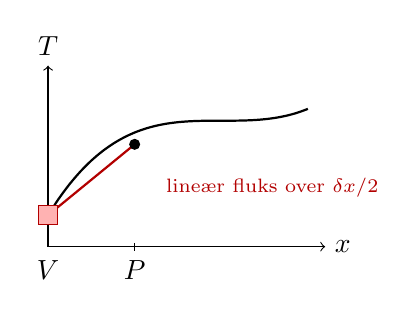
\begin{tikzpicture}[x=1.1cm,y=1cm]
\draw[->] (0,0) -- (3.2,0) node[right] {$x$};
\draw[->] (0,0) -- (0,2.3) node[above] {$T$};
\draw[thick, domain=0:3, smooth] plot (\x, {0.4+1.8*\x-0.9*\x*\x+0.15*\x*\x*\x});
\draw[thick, red!70!black] (0,0.4) -- (1,1.3);
\node[randpkt] at (0,0.4) {};
\fill (1,1.3) circle (2pt);
\draw (1,0.05) -- (1,-0.05) node[below] {$P$};
\node[below] at (0,-0.05) {$V$};
\node[font=\scriptsize, red!70!black, anchor=west] at (1.25,0.75) {lineær fluks over $\delta x/2$};
\end{tikzpicture}
\end{center}
\end{column}
\begin{column}{0.48\textwidth}
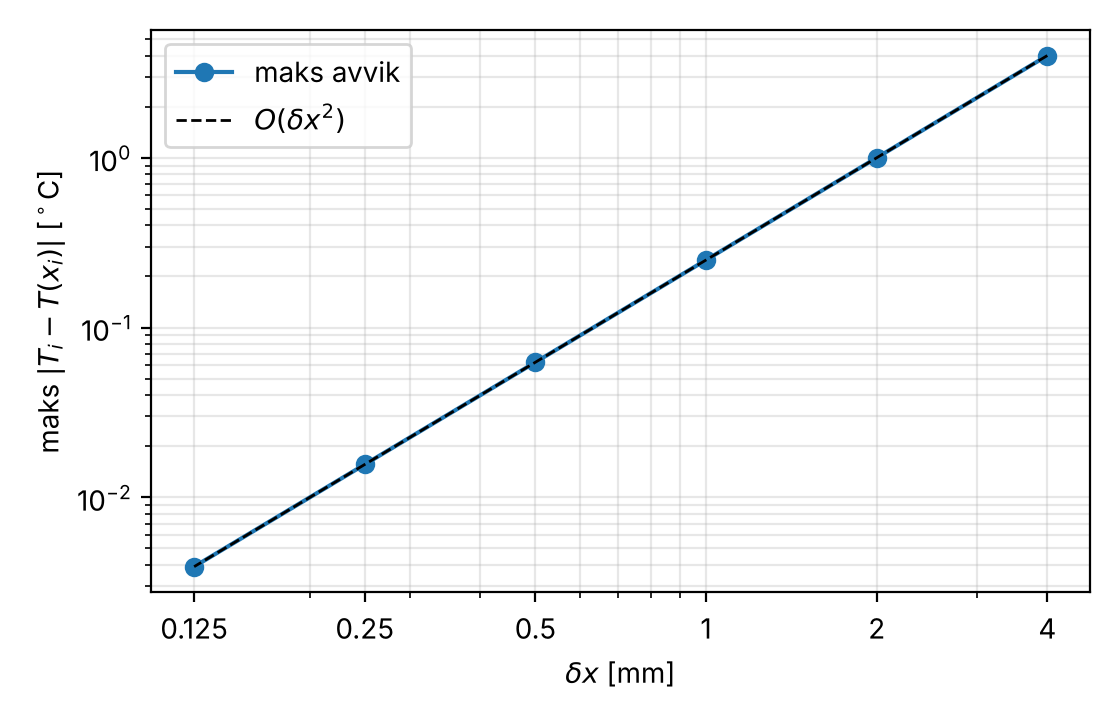
\includegraphics[width=\textwidth]{assets/konvergens.png}
\begin{oppsumb}{Avviket}
\[
\text{avvik} = \frac{q\,\delta x^2}{8k} = 4\,^\circ\text{C} \quad\Rightarrow\quad O(\delta x^2)
\]
\end{oppsumb}
\end{column}
\end{columns}
\end{frame}

\section{Eksempel: ribbe}

\begin{frame}{Eksempel: ribbe som kjøles av luft (øving 7)}
\[
\frac{d^2T}{dx^2} - n^2(T - T_\infty) = 0, \qquad n^2 = \frac{hO}{\kappa A} = 25~\text{m}^{-2}
\]
\begin{itemize}
\item Varmetapet til luften er en \textbf{sluk} som øker med $T$ $\Rightarrow$ den $T$-avhengige delen går i $S_P$:
\[
S^u = n^2\,\delta x\,T_\infty, \qquad S_P = -n^2\,\delta x \qquad (\text{etter divisjon med } A).
\]
\item Basen har kjent temperatur $T_V = 100\,^\circ$C: halv celle, som i F23.
\item Enden er \emph{isolert}: ingen fluks ut $\Rightarrow$ en ny type randbetingelse (neste slide).
\end{itemize}
\begin{remb}{Øving 7}
Dette er \texttt{EVM\_oppgave.ipynb}: sett opp \texttt{koeff\_diag}, \texttt{koeff\_over}, \texttt{koeff\_under} og \texttt{F}, løs med \texttt{la.solve(L, F)}, og sammenlign med den analytiske løsningen.
\end{remb}
\end{frame}

\section{Randbetingelser med kjent fluks}

\begin{frame}{Randbetingelse med kjent fluks (Neumann)}
\begin{center}
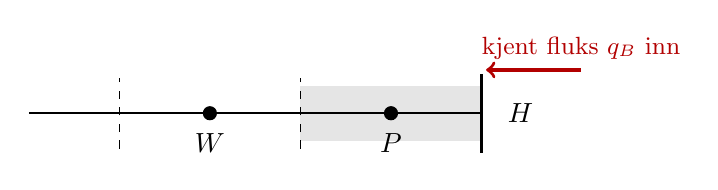
\begin{tikzpicture}[x=1.15cm]
\fill[gray!20] (3,-0.35) rectangle (5,0.35);
\draw[thick] (0,0) -- (5,0);
\draw[very thick] (5,-0.5) -- (5,0.5); \draw[dashed] (1,-0.45) -- (1,0.45); \draw[dashed] (3,-0.45) -- (3,0.45);
\node[node1d] at (2,0) {}; \node[below=4pt] at (2,0) {$W$};
\node[node1d] at (4,0) {}; \node[below=4pt] at (4,0) {$P$};
\node[right=6pt] at (5,0) {$H$};
\draw[<-, very thick, red!70!black] (5.05,0.55) -- (6.1,0.55) node[above, font=\small] {kjent fluks $q_B$ inn};
\end{tikzpicture}
\end{center}
Fluksleddet på randflaten $e$ er \emph{kjent} -- ingen tilnærming nødvendig:
\[
\underbrace{\left(kA\frac{dT}{dx}\right)_e}_{=\,q_B A} - kA\frac{T_P-T_W}{\delta x} + \overline S\,A\,\delta x = 0 .
\]
\begin{oppsumb}{Kjent fluks $q_B$ inn gjennom randen}
\[
a_E = 0, \qquad S^u \mathrel{+}= q_B A, \qquad S_P \text{ uendret}
\]
\textbf{Isolert rand:} $q_B = 0$ $\Rightarrow$ randen bidrar ikke med noe -- bare kutt koblingen.
\end{oppsumb}
\end{frame}

\begin{frame}{Eksempel: platen med isolert høyre side -- eller fluks inn}
\begin{columns}[c]
\begin{column}{0.55\textwidth}
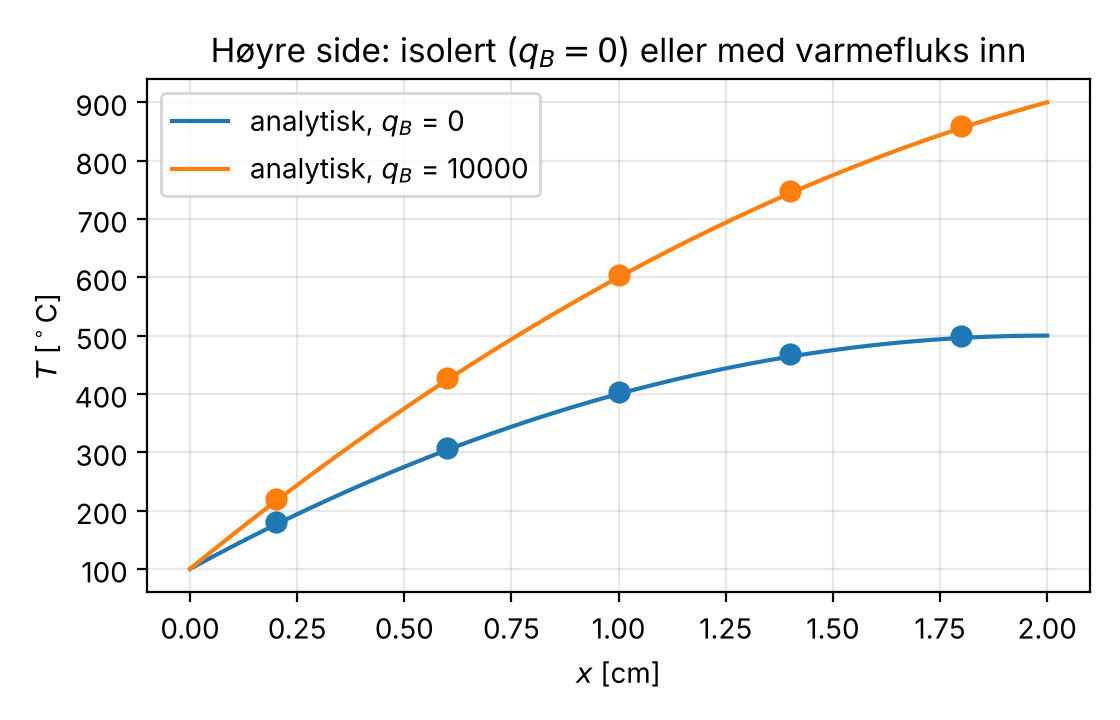
\includegraphics[width=\textwidth]{assets/fluks_rand.png}
\end{column}
\begin{column}{0.43\textwidth}
\small
$T(0)=T_V$, \; $k\,T'(R) = q_B$:
\[
T = T_V + \frac{qR+q_B}{k}x - \frac{q}{2k}x^2
\]
\textbf{Energibalanse} (5 kontrollvolum):
\begin{center}
\begin{tabular}{ccc}
\toprule
$q_B$ & ut til venstre & $qRA + q_BA$ \\
\midrule
0 & 20\,000 W & 20\,000 W \\
$10^4$ & 30\,000 W & 30\,000 W \\
\bottomrule
\end{tabular}
\end{center}
Eksakt -- selv om temperaturene har et avvik på $4\,^\circ$C.
\end{column}
\end{columns}
\end{frame}

\begin{frame}{Oppsummering: hvor havner hvert bidrag?}
\begin{center}
\renewcommand{\arraystretch}{1.4}
\begin{tabular}{lccc}
\toprule
Bidrag & nabokoeffisient & $S^u$ & $S_P$ \\
\midrule
Indre kobling & $a_W = a_E = \frac{\Gamma A}{\delta x}$ & -- & -- \\
Konstant kilde $q$ & -- & $+\,qA\,\delta x$ & -- \\
Sluk $-n^2(T-T_\infty)$ & -- & $+\,n^2 T_\infty A\,\delta x$ & $-\,n^2 A\,\delta x$ \\
Kjent randverdi $\phi_B$ & randsiden $=0$ & $+\,\frac{2\Gamma A}{\delta x}\phi_B$ & $-\,\frac{2\Gamma A}{\delta x}$ \\
Kjent randfluks $q_B$ (inn) & randsiden $=0$ & $+\,q_B A$ & -- \\
Isolert rand & randsiden $=0$ & -- & -- \\
\bottomrule
\end{tabular}
\end{center}
\begin{itemize}
\item Alltid: $a_P = a_W + a_E - S_P$, og $S_P\le0$.
\item Energibalansen er oppfylt eksakt; feilen i temperaturene er $O(\delta x^2)$.
\end{itemize}
\end{frame}

\begin{frame}{Koding: \texttt{F24\_EVM\_1D\_Kilder\_Randbetingelser.ipynb}}
\begin{enumerate}
\item \textbf{Plate-eksempelet «for hånd»:} \texttt{koeff\_diag}, \texttt{koeff\_over}, \texttt{koeff\_under}, \texttt{F} og \texttt{la.solve(L, F)} -- som i øvingen.
\item \textbf{En generell 1D-løser} \texttt{evm\_1d} med kildeledd og valgfri randbetingelse (\texttt{"T"} eller \texttt{"fluks"}).
\item \textbf{Konvergens:} vis at avviket er $q\,\delta x^2/(8k)$.
\item \textbf{Kjent fluks og energibalanse.}
\item \textbf{Hvorfor $S_P\le0$:} Jacobi med og uten $S_P$.
\end{enumerate}
\begin{remb}{Prøv selv (i notatboken)}
Variabel kilde $q_0\sin(\pi x/R)$ \;$\cdot$\; fluks \emph{ut} \;$\cdot$\; begge ender isolert -- hva skjer, og hvorfor?
\end{remb}
\end{frame}

\begin{frame}{Neste gang: F25 -- endelig volum i 2D}
\begin{nestefb}
\begin{itemize}
\item Fire naboer $W,E,S,N$ og fire flater $w,e,s,n$.
\item Randceller og hjørneceller.
\item Sammenhengen med fempunktsformelen og Jacobi/Gauss-Seidel fra F21.
\item Koding: en 2D-løser, varmekart og energibalanse.
\end{itemize}
\end{nestefb}
\end{frame}

\end{document}
